% Do NOT change this "Section" title
% and do NOT add more "Section" level titles.
\section{Method}\label{sec:method}
\subsection{System architecture}
The system needed to be able to execute missions and receive new missions through the umbilical chord. In order to do this, several tasks were set up. The new missions needed to be received using TCP, so a task was created to handle this. Missions need to communicate with the rest of the AUV through CAN, so two tasks were created to handle the input and output over CAN. Finally, a main task was created to be in charge of executing the actual missions.

\pageref{fig:data_flow_figure}
\begin{figure}[h]
    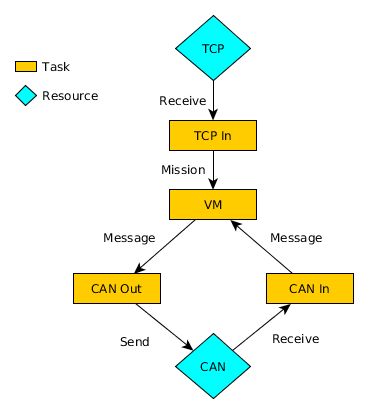
\includegraphics[width=0.5\textwidth]{./figure/figureTasksAndResources.png}
    \caption{Tasks and resources of the mission control system}
    \label{fig:data_flow_figure}
\end{figure}

\subsubsection{Virtual Machine}
The task running the virtual machine is the one responsible for executing the missions. Missions consist of stack machine code, which is interpreted by the virtual machine. Each iteration, the virtual machine runs one instruction of the mission.

\subsubsection{TCP In}
The task handling TCP input is responsible for receiving mission through the TCP resource. The task is listening on a specific port for incoming connections. When a connection is established, the task tries to receive a mission file. When the task has successfully received a mission file, a flag is set to indicate this. The virtual machine task checks for this flag each iteration, and if the flag is set, the new mission file is loaded and executed.

\subsubsection{CAN In}
The task handling CAN input is responsible for receiving CAN messages from different components in the AUV through the CAN resource. The messages are put in a list which is shared with the virtual machine task, allowing missions to retreive data from other components of the AUV.

\subsubsection{CAN Out}
The task handling CAN output is responsible for sending CAN messages to different components in the AUV through the CAN resource. The messages are retreived from a list which is shared with the virtual machine task, allowing missions to send data to other components of the AUV.
